\documentclass[a4paper]{book}
\usepackage[utf8]{vietnam}
\usepackage{xcolor}
\usepackage{titlesec}
\usepackage{mdframed}
\usepackage{amsmath}
\usepackage{placeins}
\usepackage{array}
\usepackage[amsmath,standard,thmmarks]{ntheorem}
\usepackage{amssymb}
\usepackage{exscale}
\usepackage{amsfonts}
\usepackage{eucal}
\usepackage{enumerate}
\usepackage{enumitem}
\usepackage{commath}
\usepackage{graphicx}
\usepackage{tcolorbox}
\usepackage{float}
\usepackage{subfig}
\usepackage{url}

\usepackage{scrextend}
\changefontsizes{13pt}

\usepackage{indentfirst}
\setlength{\parindent}{20pt}

\usepackage[unicode]{hyperref}
\newmdenv[linecolor=black,skipabove=\topsep,skipbelow=\topsep,
leftmargin=-5pt,rightmargin=-5pt,
innerleftmargin=5pt,innerrightmargin=5pt]{mybox}
\usepackage[left=2cm,right=2cm,top=2.5cm,bottom=2.5cm]{geometry}
\renewcommand{\baselinestretch}{1.5}
\newcommand{\heva}[1]{\left\{ 
	\begin{aligned}#1\end{aligned}\right.}

\counterwithin{figure}{section}
\counterwithin{table}{section}
\counterwithin{equation}{section}

\usepackage{fancyhdr}
\pagestyle{fancy}
\fancyhf{}
\lhead{Mô hình hóa Thống kê}
\cfoot{\thepage}
\rhead{Nhóm 4}
\title{Tiểu luận cuối kỳ}

\allowdisplaybreaks

\author{NHÓM 4}

\date{\today}%

\begin{document}
	
	\begin{titlepage}
		\thispagestyle{empty}
		\begin{center}
			\textbf{\large{ĐẠI HỌC QUỐC GIA TP. HỒ CHÍ MINH\\TRƯỜNG ĐẠI HỌC KHOA HỌC TỰ NHIÊN}}\\
			---------------*---------------\\
			\vspace*{5.5cm}
			{\textcolor[rgb]{0.0,0.0,1.0}{\textbf{\Large{TIỂU LUẬN CUỐI KÌ}}}}\\
			\vspace{1cm}
			\textbf{\huge{\textcolor[rgb]{1.0,0.0,0.0}{MÔ HÌNH HÓA THỐNG KÊ}}}\\
			\vspace*{4cm}
			\begin{tabular}{rll}
				{Giảng viên hướng dẫn:} &{\bf TS. Nguyễn Thị Mộng Ngọc} &  \\
				{Nhóm thực hiện:}     & {\textbf{Nhóm 4}} & \\
				{Học viên:} & {\textbf{Phan Thị Thùy An}} &{MSHV: 20C29002} \\
				& {\textbf{Đinh Thị Nữ }} &{MSHV: 20C29013} \\
				& {\textbf{Lý Phi Long}} &{MSHV: 20C29028} \\
				& {\textbf{Đặng Khánh Thi}} &{MSHV: 20C29038} 
			\end{tabular}
			\vfill
			\normalsize{TP. Hồ Chí Minh $-$ Tháng 04, 2021}
		\end{center}
	\end{titlepage}
\tableofcontents

\chapter{Dữ liệu tự chọn}
\begin{itemize}
	\item Tên "đề tài", nguồn gốc của dữ liệu, giới thiệu các biến.
	\item Mô hình chọn được; phân tích kết quả
	\item Đưa ra những phương pháp/phân tích khác có thể giúp cho kết quả tốt hơn.
	\item Kết luận.
\end{itemize}

\section{Dữ liệu 1: Mô hình hồi quy đa biến}

\subsection*{Giới thiệu bộ dữ liệu}
Bộ dữ liệu được tìm thấy trên trang Kaggle - một cộng đồng trực tuyến về khoa học dữ liệu và học máy. Đó là bộ dữ liệu \textbf{Chi phí Y tế Cá nhân} \footnote{\url{https://www.kaggle.com/mirichoi0218/insurance}} (\textit{Medical Cost Personal Datasets}). Đây là một bộ dữ liệu được lấy ra từ cuốn \textit{Machine Learning with R} của Brett Lantz, một cuốn sách giới thiệu về học máy bằng R.

Bộ dữ liệu ghi lại các thông tin về thông tin của người đăng kí bảo hiểm và chi phí mà bảo hiểm y tế phải chi trả cho cá nhân người đó. Bộ dữ liệu có 1338 quan trắc, gồm 7 biến sau:
\begin{enumerate}
	\item \textbf{Age}: age of primary beneficiary
	\item \textbf{Sex}: giới tính của người đăng kí bảo hiểm
	\item \textbf{BMI}: Body mass index, providing an understanding of body, weights that are relatively high or low relative to height,	objective index of body weight ($kg / m ^ 2$) using the ratio of height to weight, ideally 18.5 to 24.9
	\item \textbf{Children}: số lượng trẻ em phụ thuộc được bao gồm bởi bảo hiểm y tế.	
	\item \textbf{Smoker}: 1 nếu người đó có hút thuốc, ngược lại là 0.
	\item \textbf{Region}: the beneficiary's residential area in the US, northeast, southeast, southwest, northwest.
	\item \textbf{Charges}: Chi phí y tế chi trả cho cá nhân được chi bởi bảo hiểm y tế.
\end{enumerate}

\subsection*{Phân tích và chọn mô hình}

\subsection*{Nhận xét và kết luận}
\section{Dữ liệu 2: Hồi quy thành phần chính}

\subsection*{Giới thiệu bộ dữ liệu}
Hiện nay, Xe đạp cho thuê được giới thiệu ở nhiều thành phố để nâng cao sự thoải mái khi di chuyển. Điều cần quan tâm khi cho thuê xe đạp là xe đạp phải luôn sẵn sàng và tiếp cận được người dùng vào đúng thời điểm, giúp giảm bớt thời gian chờ. Do đó, việc đảm bảo một nguồn cung cấp xe đạp cho thuê ổn định cho thành phố trở thành mối quan tâm lớn. Phần quan trọng là cần dự đoán được số lượng xe đạp cần thiết tại mỗi giờ, để có được nguồn cung cấp xe đạp cho thuê ổn định.

Nhóm em sử dụng bộ dữ liệu Nhu cầu thuê xe đạp ở Seoul\footnote{\url{https://archive.ics.uci.edu/ml/datasets/Seoul+Bike+Sharing+Demand}} (\textbf{Seoul Bike Sharing Demand Dataset}).

Bộ dữ liệu ghi lại các thông tin về thời tiết, số lượng xe đạp được thuê mỗi giờ theo từng ngày, từ 01/12/2017 đến 31/11/2018. Bộ dữ liệu có 8760 quan trắc, gồm 14 biến sau:
\begin{enumerate}
	\item \textbf{Date} - Ngày ghi lại số lượng xe đạp cho thuê
	\item \textbf{Rented Bike count} - Số lượng xe đạp được thuê được ghi lại theo mỗi giờ
	\item \textbf{Hour} - Giờ trong ngày
	\item \textbf{Temperature} - Nhiệt độ ($^o C$)
	\item \textbf{Humidity} - Độ ẩm (\%)
	\item \textbf{Windspeed} - Tốc độ gió ($m/s$)
	\item \textbf{Visibility} - Tầm nhìn xa ($10m$)
	\item \textbf{Dew point temperature} - Nhiệt độ điểm sương ($^o C$)
	\item \textbf{Solar radiation} - Bức xạ mặt trời ($Mj/m^2$)
	\item \textbf{Rainfall} - Lượng mưa ($mm$)
	\item \textbf{Snowfall} - Lượng tuyết rơi ($cm$)
	\item \textbf{Seasons} - Mùa (Winter, Spring, Summer, Autumn)
	\item \textbf{Holiday} - Ngày lễ (Holiday/No holiday)
	\item \textbf{Functional Day} - Ngày làm việc (Yes nếu là ngày làm việc, No nếu ngược lại)
\end{enumerate}


\subsection*{Phân tích và chọn mô hình}

\subsection*{Nhận xét và kết luận}

\chapter{Dữ liệu có sẵn}
\begin{itemize}
	\item Chọn mô hình phù hợp nhất giải thích biến phụ thuộc với từng bộ dữ liệu.
	\item Nêu rõ phương pháp chọn mô hình và lý do chọn phương pháp đó.
	\item Nói rõ ý nghĩa của mô hình đã chọn.
\end{itemize}

\section{Dữ liệu 1}
Những thông tin vê các giám đốc điều hành các tập đoàn Hoa Kỳ. Bộ dữ liệu gồm 177 quan trắc và 15 biến.

$*$ \textbf{Phương pháp chọn: Stepwise - tiến; tiêu chuẩn chọn: AIC}.

\subsection*{Tìm hiểu và tiền xử lý dữ liệu}

Một số biến trong bộ dữ liệu kiểu số có đơn vị tính lớn như: \texttt{sales}, \texttt{profit}, \texttt{lmktval}. Nếu đưa những biến này vào phương trình hồi quy có thể dẫn tới hiện tượng bias do tác~động của những biến này lên model lấn át những biến khác còn lại như $age$, $ceoten$.... Nên ta sẽ dùng phương pháp logarit cho 3 biến này trong model tương ứng với 3 biến mới là:  $lsales$, $lmktval$ và $profmarg$. (1) \label{abc}

Từ biểu đồ dưới ta thấy ba biến định lượng $\textit{lsales}$, $\textit{lmktval}$ và $\textit{profmarg}$ xảy ra hiện~tượng đa cộng tuyến.
Tuy nhiên có xảy ra hiện tượng đa cộng tuyến giữa 2 biến \texttt{sales} và \texttt{profit} (hình \ref{fig-b1:plot-vars}).

Tính độ tương quan giữa biến $salary$ với lần lượt 2 biến trên ta có:

\begin{figure}[H]
	\centering
	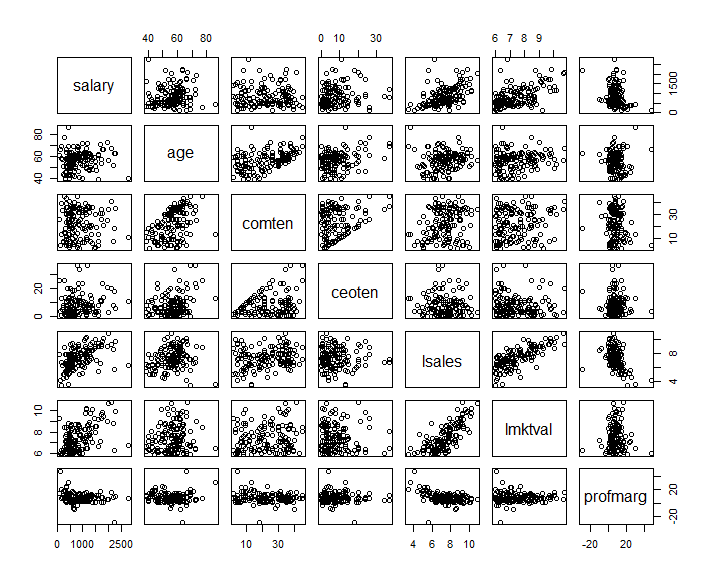
\includegraphics[width=.7\linewidth]{../Photo Of Result/B1_plotVriables.png}  
	\caption{Mối tương quan giữa các biến}
	\label{fig-b1:plot-vars}
\end{figure}

\begin{figure}[H]
	\centering
	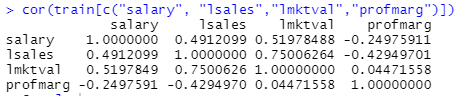
\includegraphics[width=.7\linewidth]{../Photo Of Result/B1_CorTable.PNG}  
	\caption{Mức độ tương quan giữa biến \texttt{lsales} và \texttt{promarg}}
	\label{fig-b1:corr-table}
\end{figure}

Xét bảng correlation giữa các biến độc lập với nhau và giữa các biến độc lập với biến phụ thuộc, ta thấy: Giữa hai biến $\textit{lmktval}$ và biến $\textit{lsales}$ có mối tương quan rất cao ($\approx$ 0.75). Tuy nhiên biến $\textit{lmktval}$ lại có mối tương quan cao hơn với biến phụ thuộc $\textit{salary}$. Mặt khác giữa biến $\textit{profmarg}$ và $\textit{lsales}$ cũng có mối tương quan cao ($\approx -0.42$). Nên ta loại bỏ biến $\textit{lsales}$ khỏi danh sách các biến được xét. (2)

Từ (1) và (2) ta có mô hình với đầy đủ các biến cần lựa chọn như sau:
\begin{equation}\label{eq-b1:full-model}
	\begin{split}
		salary 	= \beta_0 + &\beta_1 \times age + \beta_2 \times college + \beta_3 \times grad + \beta_4 \times comten\\
		+ &\beta_5\times ceoten + \beta_6\times lmktval + \beta_7\times profmarg
	\end{split}
\end{equation}


Thực hiện phân rã hai biến phân loại gồm $college$ và $grad$ trước khi thực hiện phương pháp  \textbf{Stepwise} \textbf{tiến} với \textbf{tiêu chuẩn AIC}.

Để đánh giá chất lượng mô hình ta chia tâp dữ liệu thành hai phần, training và testing, với tỷ lệ $8:2$ sau đó tiến hành phương pháp chọn biến trên tập training.

\subsection*{Chọn biến bằng phương pháp Stepwise tiến và tiêu chuẩn AIC}

\begin{figure}[H]
	\centering
	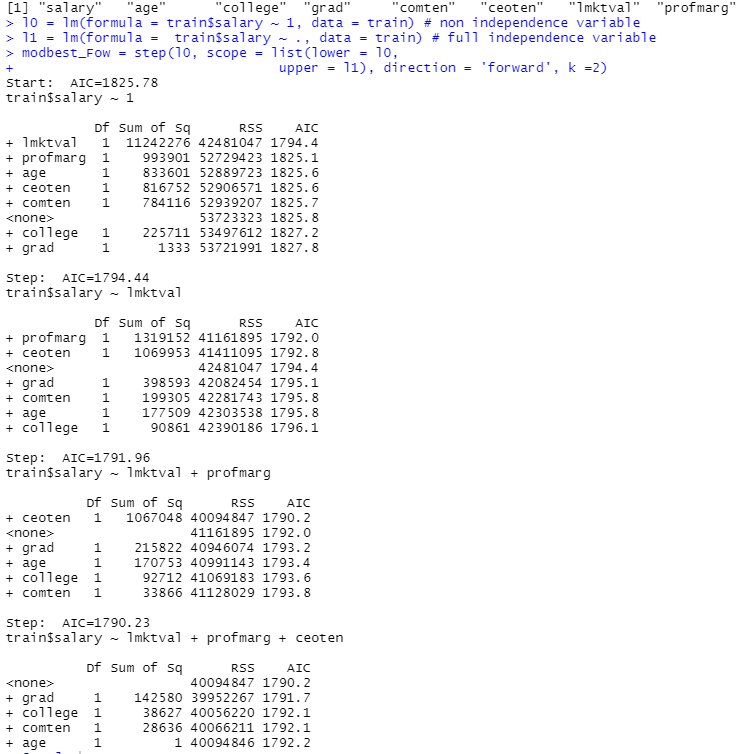
\includegraphics[width=\linewidth]{../Photo Of Result/B1_stepwiseForward.PNG}  
	\caption{Kết quả chọn biến theo phương pháp StepWise tiến với tiêu chuẩn AIC}
	\label{fig-b1:stepwise-forward}
\end{figure}

Tổng quan tiêu chuẩn AIC thì mô hình tốt là mô hình có giá trị AIC nhỏ nhất. Ở mô hình 1, biến $\textit{lmktval}$ được chọn vào mô hình vì có AIC nhỏ nhất trong tất cả các kết~hợp với các biến còn lại. Tương tự AIC được tính cho mô hình thêm biến thứ 2, $\textit{ceoten}$, và biến thứ 3 là $\textit{ceoten}$ (hình \ref{ex1:model:1}).

\begin{figure}[H]
	\centering
	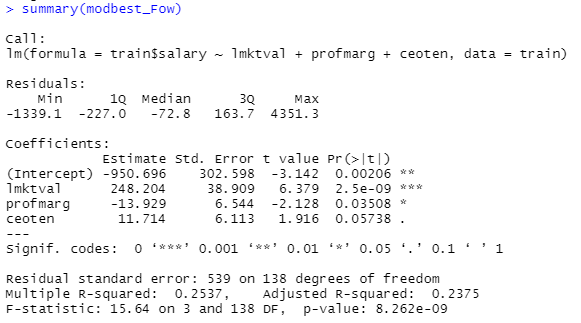
\includegraphics[width=.7\linewidth]{../Photo Of Result/B1_summary.PNG}  
	\caption{Kết quả hồi quy mô hình với các biến được chọn}
	\label{ex1:model:1}
\end{figure}

Với ba biến được chọn ở trên, mô hình \ref{eq-b1:full-model} trở thành mô hình mới:
\begin{equation}\label{1.2}
\textit{salary} = -950.6 + 248.2 * \textit{lmktval} - 13.9 *\textit{profmarg} + 11.7  *\textit{ceoten}
\end{equation}

Tuy nhiên ta nhận thấy biến $\textit{ceoten}$ có $\rho_{value} \ge \alpha$ (0.05738 $\ge$ 0.05) nên không có ý~nghĩa thống kê trong mô hình. Ta tiến hành bỏ biến $\textit{ceoten}$ và hồi quy mô hình với hai biến còn lại kết quả thu được từ phần mềm R như hình \ref{fig-b1:new-summary}:

\begin{figure}[H]
	\centering
	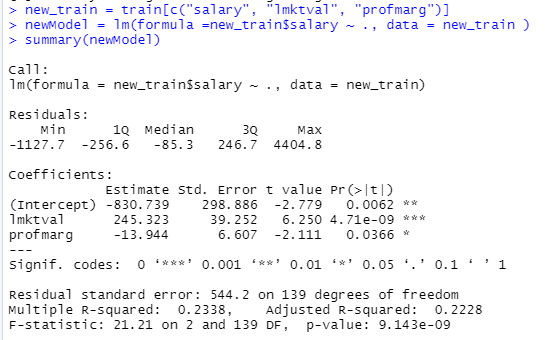
\includegraphics[width=.7\linewidth]{../Photo Of Result/B1_newsummary.PNG}  
	\caption{Kết quả hồi quy mô hình với hai biến còn lại}
	\label{fig-b1:new-summary}
\end{figure}

Mô hình thống kê mới:
\begin{equation}\label{1.3}
\textit{salary} = -830.7 + 245.3 *\textit{lmktval} -13.9 *\textit{profmarg}
\end{equation}

Trường hợp này hai biến còn lại có ý nghĩa thống kê. Tuy nhiên mô hình được tạo bởi hai biến này chỉ giải thích được 23$\%$ sự biến thiên của biến phụ thuộc (hình \ref{fig-b1:new-summary}). Nguyên nhân dẫn tới kết quả thấp là do số lượng data ít, các biến giải thích ít không tạo nên mô hình đặc trưng được.

\subsection*{Test trên tập test và nhận xét kết quả}

Thực hiện dự đoán trên tập dữ liệu test từ kết quả mô hình \ref{1.3} và dùng chỉ số đánh giá MSE (trung bình bình phương sai số) ta có:

\begin{figure}[H]
	\centering
	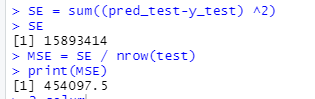
\includegraphics[width=.5\linewidth]{../Photo Of Result/B1_MSE.PNG}  
	\caption{Chỉ số đo lường kết quả MSE}
	\label{fig-b1:mse}
\end{figure}

Kết quả MSE $\approx$ 454097 lớn hơn nhiều so với giá trị Mean : 887.5 nên ta có thể thấy hai yếu tố gồm: giá thị trường (\textit{lmktval}) và tỷ lệ phần trăm lợi nhuận (\textit{profmarg}) là chưa đủ để giải thích mức độ tăng giảm của tiền lương của các giám đốc điều hành các tập~đoàn Hoa Kỳ. 

Để cải thiện kết quả mô hình ta nên tiến hành thu thập thêm dữ liệu và tiến hành lựa chọn biến dựa trên dữ liệu mới này. Bên cạnh đó có thể xem xét tới xem xét tới các nhân tố khác ảnh hưởng tới tiền lương của các giám đốc Hoa kỳ như: Lĩnh vực hoạt~động (ngân hàng, hàng không, công nghệ, vận tải...); mức lương trước đó; số năm kinh nghiệm, giới tính,...
	


\documentclass[a4paper]{article}
\usepackage[utf8]{vietnam}
\usepackage{scrextend}
\changefontsizes{13pt}
\usepackage{xcolor}
\usepackage{titlesec}
\usepackage{mdframed}
\usepackage{amsmath}
\usepackage{placeins}
\usepackage{array}
\usepackage[amsmath,standard,thmmarks]{ntheorem}
\usepackage{amssymb}
\usepackage{exscale}
\usepackage{amsfonts}
\usepackage{eucal}
\usepackage{enumerate}
\usepackage{enumitem}
\usepackage{commath}
\usepackage{graphicx}
\usepackage{tcolorbox}
\usepackage{url}
\usepackage[unicode]{hyperref}
\newmdenv[linecolor=black,skipabove=\topsep,skipbelow=\topsep,
leftmargin=-5pt,rightmargin=-5pt,
innerleftmargin=5pt,innerrightmargin=5pt]{mybox}
\setlength{\parindent}{0pt}
\usepackage[left=2cm,right=2cm,top=2.5cm,bottom=2.5cm]{geometry}
\renewcommand{\baselinestretch}{1.5}
\newcommand{\heva}[1]{\left\{ 
	\begin{aligned}#1\end{aligned}\right.}
\usepackage{fancyhdr}
\pagestyle{fancy}
\fancyhf{}
\lhead{Xử lý ngôn ngữ tự nhiên}
\cfoot{\thepage}
\rhead{Tương đồng văn bản}
\title{Tiểu luận NLP}

\allowdisplaybreaks

\author{NHÓM 4}

\date{\today}%

\begin{document}
	
	\begin{titlepage}
		\thispagestyle{empty}
		\begin{center}
			\textbf{\large{ĐẠI HỌC QUỐC GIA TP. HỒ CHÍ MINH\\TRƯỜNG ĐẠI HỌC KHOA HỌC TỰ NHIÊN}}\\
			---------------*---------------\\
			\vspace*{5cm}
			{\textcolor[rgb]{0.0,0.0,1.0}{\textbf{TIỂU LUẬN XỬ LÝ NGÔN NGỮ TỰ NHIÊN}}}\\
			\vspace{1.5cm}
			\textbf{\huge{\textcolor[rgb]{1.0,0.0,0.0}{TƯƠNG ĐỒNG VĂN BẢN \\ CẤP ĐỘ CÂU}}}\\
			\vspace*{4cm}
			$\begin{array}{rl}
				\text{Giảng viên hướng dẫn:} &\text{\bf PGS.TS. Đinh Điền}  \\
				\text{Giảng viên trợ giảng:} &\text{\bf NCS. Lương An Vinh}  \\
				\text{Nhóm thực hiện:}     & \text{\textbf{Nhóm 14}}\\
				\text{Học viên:} & \text{\textbf{Đinh Thị Nữ }- MSHV: 20C29013} \\
				& \text{\textbf{Vũ Đức Hiếu} - MSHV: 20C29006} \\
				& \text{\textbf{Phan Thị Thùy An} - MSHV: 20C29002} 
			\end{array}$\\
			\vfill
			\normalsize{TP. Hồ Chí Minh $-$ Tháng 03, 2021}
		\end{center}
	\end{titlepage}
\tableofcontents
\include{GioiThieu}
\include{HuongNC}
\include{reference}
\include{BangPhanCong}
\end{document}
\documentclass[a4paper]{article}
\usepackage[utf8]{vietnam}
\usepackage{scrextend}
\changefontsizes{13pt}
\usepackage{xcolor}
\usepackage{titlesec}
\usepackage{mdframed}
\usepackage{amsmath}
\usepackage{placeins}
\usepackage{array}
\usepackage[amsmath,standard,thmmarks]{ntheorem}
\usepackage{amssymb}
\usepackage{exscale}
\usepackage{amsfonts}
\usepackage{eucal}
\usepackage{enumerate}
\usepackage{enumitem}
\usepackage{commath}
\usepackage{graphicx}
\usepackage{tcolorbox}
\usepackage{url}
\usepackage[unicode]{hyperref}
\newmdenv[linecolor=black,skipabove=\topsep,skipbelow=\topsep,
leftmargin=-5pt,rightmargin=-5pt,
innerleftmargin=5pt,innerrightmargin=5pt]{mybox}
\setlength{\parindent}{0pt}
\usepackage[left=2cm,right=2cm,top=2.5cm,bottom=2.5cm]{geometry}
\renewcommand{\baselinestretch}{1.5}
\newcommand{\heva}[1]{\left\{ 
	\begin{aligned}#1\end{aligned}\right.}
\usepackage{fancyhdr}
\pagestyle{fancy}
\fancyhf{}
\lhead{Xử lý ngôn ngữ tự nhiên}
\cfoot{\thepage}
\rhead{Tương đồng văn bản}
\title{Tiểu luận NLP}

\allowdisplaybreaks

\author{NHÓM 4}

\date{\today}%

\begin{document}
	
	\begin{titlepage}
		\thispagestyle{empty}
		\begin{center}
			\textbf{\large{ĐẠI HỌC QUỐC GIA TP. HỒ CHÍ MINH\\TRƯỜNG ĐẠI HỌC KHOA HỌC TỰ NHIÊN}}\\
			---------------*---------------\\
			\vspace*{5cm}
			{\textcolor[rgb]{0.0,0.0,1.0}{\textbf{TIỂU LUẬN XỬ LÝ NGÔN NGỮ TỰ NHIÊN}}}\\
			\vspace{1.5cm}
			\textbf{\huge{\textcolor[rgb]{1.0,0.0,0.0}{TƯƠNG ĐỒNG VĂN BẢN \\ CẤP ĐỘ CÂU}}}\\
			\vspace*{4cm}
			$\begin{array}{rl}
				\text{Giảng viên hướng dẫn:} &\text{\bf PGS.TS. Đinh Điền}  \\
				\text{Giảng viên trợ giảng:} &\text{\bf NCS. Lương An Vinh}  \\
				\text{Nhóm thực hiện:}     & \text{\textbf{Nhóm 14}}\\
				\text{Học viên:} & \text{\textbf{Đinh Thị Nữ }- MSHV: 20C29013} \\
				& \text{\textbf{Vũ Đức Hiếu} - MSHV: 20C29006} \\
				& \text{\textbf{Phan Thị Thùy An} - MSHV: 20C29002} 
			\end{array}$\\
			\vfill
			\normalsize{TP. Hồ Chí Minh $-$ Tháng 03, 2021}
		\end{center}
	\end{titlepage}
\tableofcontents
\include{GioiThieu}
\include{HuongNC}
\include{reference}
\include{BangPhanCong}
\end{document}
\documentclass[a4paper]{article}
\usepackage[utf8]{vietnam}
\usepackage{scrextend}
\changefontsizes{13pt}
\usepackage{xcolor}
\usepackage{titlesec}
\usepackage{mdframed}
\usepackage{amsmath}
\usepackage{placeins}
\usepackage{array}
\usepackage[amsmath,standard,thmmarks]{ntheorem}
\usepackage{amssymb}
\usepackage{exscale}
\usepackage{amsfonts}
\usepackage{eucal}
\usepackage{enumerate}
\usepackage{enumitem}
\usepackage{commath}
\usepackage{graphicx}
\usepackage{tcolorbox}
\usepackage{url}
\usepackage[unicode]{hyperref}
\newmdenv[linecolor=black,skipabove=\topsep,skipbelow=\topsep,
leftmargin=-5pt,rightmargin=-5pt,
innerleftmargin=5pt,innerrightmargin=5pt]{mybox}
\setlength{\parindent}{0pt}
\usepackage[left=2cm,right=2cm,top=2.5cm,bottom=2.5cm]{geometry}
\renewcommand{\baselinestretch}{1.5}
\newcommand{\heva}[1]{\left\{ 
	\begin{aligned}#1\end{aligned}\right.}
\usepackage{fancyhdr}
\pagestyle{fancy}
\fancyhf{}
\lhead{Xử lý ngôn ngữ tự nhiên}
\cfoot{\thepage}
\rhead{Tương đồng văn bản}
\title{Tiểu luận NLP}

\allowdisplaybreaks

\author{NHÓM 4}

\date{\today}%

\begin{document}
	
	\begin{titlepage}
		\thispagestyle{empty}
		\begin{center}
			\textbf{\large{ĐẠI HỌC QUỐC GIA TP. HỒ CHÍ MINH\\TRƯỜNG ĐẠI HỌC KHOA HỌC TỰ NHIÊN}}\\
			---------------*---------------\\
			\vspace*{5cm}
			{\textcolor[rgb]{0.0,0.0,1.0}{\textbf{TIỂU LUẬN XỬ LÝ NGÔN NGỮ TỰ NHIÊN}}}\\
			\vspace{1.5cm}
			\textbf{\huge{\textcolor[rgb]{1.0,0.0,0.0}{TƯƠNG ĐỒNG VĂN BẢN \\ CẤP ĐỘ CÂU}}}\\
			\vspace*{4cm}
			$\begin{array}{rl}
				\text{Giảng viên hướng dẫn:} &\text{\bf PGS.TS. Đinh Điền}  \\
				\text{Giảng viên trợ giảng:} &\text{\bf NCS. Lương An Vinh}  \\
				\text{Nhóm thực hiện:}     & \text{\textbf{Nhóm 14}}\\
				\text{Học viên:} & \text{\textbf{Đinh Thị Nữ }- MSHV: 20C29013} \\
				& \text{\textbf{Vũ Đức Hiếu} - MSHV: 20C29006} \\
				& \text{\textbf{Phan Thị Thùy An} - MSHV: 20C29002} 
			\end{array}$\\
			\vfill
			\normalsize{TP. Hồ Chí Minh $-$ Tháng 03, 2021}
		\end{center}
	\end{titlepage}
\tableofcontents
\include{GioiThieu}
\include{HuongNC}
\include{reference}
\include{BangPhanCong}
\end{document}

\end{document}